\documentclass[aspectratio=43, dvipdfmx, 12pt]{beamer}

\usepackage{graphicx}
\usepackage{amsmath}
\usepackage{amssymb}
\usepackage{bm}

\newcommand{\Real}{\mathbb{R}} % 実数空間
\newcommand{\Complex}{\mathbb{C}} % 複素空間

\newcommand{\norm}[1]{\left\|#1\right\|} % ノルム (数式モードで使用すること)
\newcommand{\vek}[1]{\bm{#1}} % ベクトル (ドイツ語は Vektor らしいので)

\newcommand{\argmax}{\mathop{\rm argmax}\limits} % argmax
\newcommand{\argmin}{\mathop{\rm argmin}\limits} % argmin
\newcommand{\vdot}[2]{\langle #1, #2 \rangle} % ベクトルの内積 \vdot{a}{b} のように使用

\usetheme{Copenhagen}
\usecolortheme{orchid}
\usefonttheme{professionalfonts}
\renewcommand{\kanjifamilydefault}{\gtdefault}

\title[機械学習の基礎概念]{機械学習輪読 I}
\author{電気通信大学大学院 修士2年 \\ 山岡 勇太}
\date{2019/09/21}

\begin{document}
\maketitle

\begin{frame}{目次}
  \tableofcontents
\end{frame}

\section{機械学習について}

\begin{frame}{目次}
  \tableofcontents[currentsection]
\end{frame}

\begin{frame}{背景}
  1990年代以降,
  \begin{itemize}
    \item インターネットの加速度的進展
    \item 計算機の処理速度
    \item ハードディスクなどの外部記憶容量の増大
  \end{itemize}
  によって, 処理対象のデータが爆発的に増加した.
  この大規模なデータ (\alert{ビッグデータ}) に対し, \alert{データマイニング}を行うことが求められるようになった.

  \begin{alertblock}{データマイニング}
    (簡単に言えば) 統計的処理などにより, 与えられたデータから有用な情報を抽出すること.
  \end{alertblock}
\end{frame}

\begin{frame}{背景}
  データマイニングの数理的モデルとして位置付けられるようになったのが\alert{機械学習}という学問分野.
\end{frame}

\section{機械学習のモデル}

\begin{frame}{目次}
  \tableofcontents[currentsection]
\end{frame}

\begin{frame}{モデルとは何か?}
  モデルとは, \alert{入力から出力を得る過程を数理的に定式化したもの}である.\\
  以降, 具体的に定義する.
\end{frame}

\begin{frame}{準備}
  とある観測者は何らかのデータ$\vek{x}$を観測する. ここで, $\vek{x}$は何らかのクラス$y$に属すものとする. クラス全体を\alert{情報源}と呼ぶ. \\
  ここで, $\vek{x}$はベクトルとする. 
  \begin{exampleblock}{具体例}
    \begin{description}
      \item[情報源 :] 新聞記事全体
      \item[$y$ :] 政治の記事, 経済の記事, スポーツの記事, etc. 
      \item[$\vek{x}$ :] 実際に書かれた記事
    \end{description}
  \end{exampleblock}
\end{frame}

\begin{frame}{予測過程}
  \begin{block}{予測過程とは?}
  観測者が新たに観測したデータ$\vek{x}$に対応する情報源のクラス$y$を知りたい場合に行う,
  ($\vek{x}$を何らかの方法で逆変換して) $y$の値を予測する計算のこと.
  \end{block}

  予測過程の結果得られた値を$\hat{y}$とする.
\end{frame}

\begin{frame}{学習過程}
  \begin{block}{学習過程とは?}
    逆変換は$y$の条件付き確率$p(y|\vek{x})$によって行われるとする. \\
    この確率密度関数$p$を求める計算のこと.
  \end{block}
  以後, 学習といえば, この学習過程を指す. また, 確率密度関数は単に確率分布と呼ぶ. 
\end{frame}

\begin{frame}{ラベル付きデータ}
  \begin{block}{ラベル付きデータとは?}
    観測されたデータ$\vek{x}$に対応する$y$が知られているとする. \\
    このような$\vek{x}$と$y$の組の集合$\mathcal{D}=\left\{(\vek{x}_{1}, y_{1}), \cdots, (\vek{x}_{n}, y_{n})\right\}$のこと.
  \end{block}
  教師データや訓練データって言ったりもする.
  \begin{alertblock}{前提}
    $\mathcal{D}$の各要素は, ある確率分布に従って独立に生成されたものとする (このとき$\mathcal{D}$は\alert{独立同一分布}に従うという).
    独立同一分布でない場合も機械学習の対象だが, テキストでは扱わない.
  \end{alertblock}
  ラベル付けは人間によって行われることが多い (らしい).
\end{frame}

\begin{frame}{予測過程のお話}
  観測したデータ$\vek{x}$から未知の$y$を推定する問題を考える.\\
  この問題は, $\vek{x}$が知られているという条件のもとでの$y$の確率,
  すなわち$p(y|\vek{x})$を最大化するような$y$の予測値$\hat{y}$を求めること.\\
  従って, 次の式で表される. 
  \begin{equation}
    \label{eq:argmax}
    \hat{y} = \argmax_{y}p(y|\vek{x})
  \end{equation}
\end{frame}

\begin{frame}{学習過程のお話}
  $y$についての事前情報がある, すなわち$\mathcal{D}$が与えられている場合について考えてみる. \\
  $\mathcal{D}$から推定される$p(\vek{x}|y)$は, $\mathcal{D}$の要素数が少ないと信頼性が低い. また, 情報源の性質である$p(y)$が使われていない (式\ref{eq:argmax}を参照).
\end{frame}

\begin{frame}{学習過程のお話 : 例}
  以下のようなラベル付きデータ$\mathcal{D}$がある.
  \[
    \mathcal{D} = \left\{ (\vek{x}_{a}, y_{1}), (\vek{x}_{b}, y_{2}), (\vek{x}_{c}, y_{3}), (\vek{x}_{a}, y_{2}), (\vek{x}_{b}, y_{3}), (\vek{x}_{a}, y_{3}) \right\}
  \]
  このとき...
  \begin{itemize}
    \item $p(y_{1}) = 1/6$
    \item $p(y_{2}) = 2/6 = 1/3$
    \item $p(y_{3}) = 3/6 = 1/2$
    \item $p(\vek{x}_{b}|y_{2}) = (1/6)/(1/3) = 1/2$
    \item $p(\vek{x}_{a}|y_{3}) = (1/6)/(1/2) = 1/3$
    \item $p(\vek{x}_{c}|y_{3}) = (1/6)/(1/2) = 1/3$
  \end{itemize}
\end{frame}

\begin{frame}{具体例}
  次のような状況を考える. この例では, 情報源のクラスは$0, 1$の2つで, 観測データも$0, 1$の2値を取るとする. 
  ここでは, 情報源出力の$0$を$1$, $1$を$0$に変換する確率は各々$0.5$とする.
  \begin{figure}[h]
    \begin{center}
      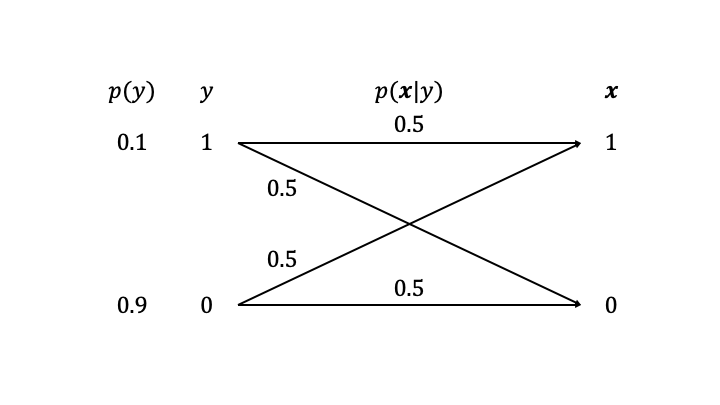
\includegraphics[scale=0.3]{./images/ML-lect1-1.png}
      \caption{情報源から観測データへの変換}
    \end{center}
  \end{figure}

\end{frame}

\begin{frame}{具体例}
  この状況下では, $p(y|\vek{x})$だけを考慮した式\ref{eq:argmax}を用いると...\\
  $0$を観測 $\Rightarrow \hat{y} = p(1|0) = p(0|0) = 0.5$. しかし$y=0$を出力する確率が高いので$\hat{y} = 0$っぽい?
  \begin{figure}[h]
    \begin{center}
      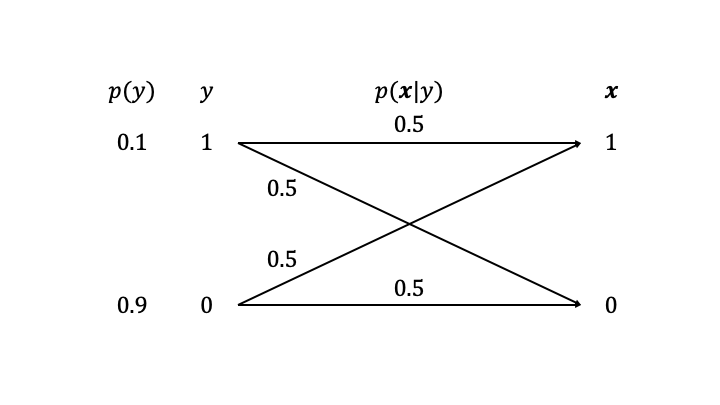
\includegraphics[scale=0.3]{./images/ML-lect1-1.png}
      \caption{情報源から観測データへの変換}
    \end{center}
  \end{figure}
\end{frame}

\begin{frame}{具体例}
  ここで\alert{ベイズの定理}を使ってみる.
  \begin{block}{定理1.1 ベイズ (Bayes) の定理}
    \[
      p(y|\vek{x}) = \frac{p(\vek{x}|y)p(y)}{\sum_{y}p(\vek{x}|y)p(y)}
    \]
  \end{block}
  $\sum_{y}p(\vek{x}|y)p(y) = p(\vek{x})$より, 次のようにも書ける.
  \begin{block}{ベイズの定理 (変形後)}
    \[
      p(y|\vek{x}) = \frac{p(\vek{x}|y)p(y)}{p(\vek{x})}
    \]
  \end{block}
\end{frame}

\begin{frame}{具体例}
  ベイズの定理より, 式\ref{eq:argmax}は次のように書ける.
  \begin{equation}
    \label{eq:newargmax}
    \hat{y} = \argmax_{y}p(\vek{x}|y)p(y)
  \end{equation}
  $\vek{x}$は観測された値であり, $y$にargmaxに関与しないので上記の式になる.\\
  式\ref{eq:newargmax}を用いることで, $p(y)$を事前知識として利用できる.\\
  この式で$0$を観測した場合の推定値を計算すると, 
  \begin{description}
    \item[$y=0$ :] $p(0|0)p(0) = 0.5 \times 0.9 = 0.45$
    \item[$y=1$ :] $p(0|1)p(1) = 0.5 \times 0.1 = 0.05$
  \end{description}
  よって, $\hat{y} = 0$.
\end{frame}

\begin{frame}{まとめ}
  \begin{itemize}
    \item 機械学習とは, データマイニングの数理的モデル.
    \item 機械学習は, 学習過程と予測過程からなる.
    \item ラベル付きデータは独立同一分布に従う (そうでないものもあるが, 今回は扱わない).
    \item (当たり前だけど) モデル化の仕方によって, 得られる結果が変わる.  
  \end{itemize}
\end{frame}

\end{document}